\chapter{平面图样绘制}
{\bfseries 知识目标}
\begin{itemize}
\item 了解国家制图标准和电气 AutoCAD 制图规范
\item 掌握平面图样的绘制步骤和方法
\item 掌握用 AutoCAD 绘制平面图样的基本步骤和方法
\item 掌握 AutoCAD 基本的绘图命令
\end{itemize}

{\bfseries 技能目标}
\begin{itemize}
\item 具备平面样抄绘能力
\item 具备使用AutoCAD绘制中等复杂程度的图样的能力
\item 具备阅读和分析平面图样的能力
\end{itemize}

{\bfseries 本章导引}

图\ref{fig:shangmu1}所示图纸即为图样,是根据投影法,并按照国家或国际标准的规定绘制的,用于工程施工或产品制造等用途的图。标准则是为了在一定范围内获得最佳秩序,而对活动或其结果规定共同的和重复使用的规则、导则或特性的文件。本章旨在通过讲解图\ref{fig:shangmu1}所示项目,使学生在完成项目的同时,了解和掌握国家制图标准中图幅、比例、线型、文字、标注等相关知识,以及通过AutoCAD进行图样绘制的步骤、方法、技巧和规范,并能运用所学的技巧和知识解决绘图过程中的实际问题,具备遵照国家制图标准和规范抄绘图样的能力。
\noindent
\begin{landscape}
\begin{figure}[htbp]
\centering
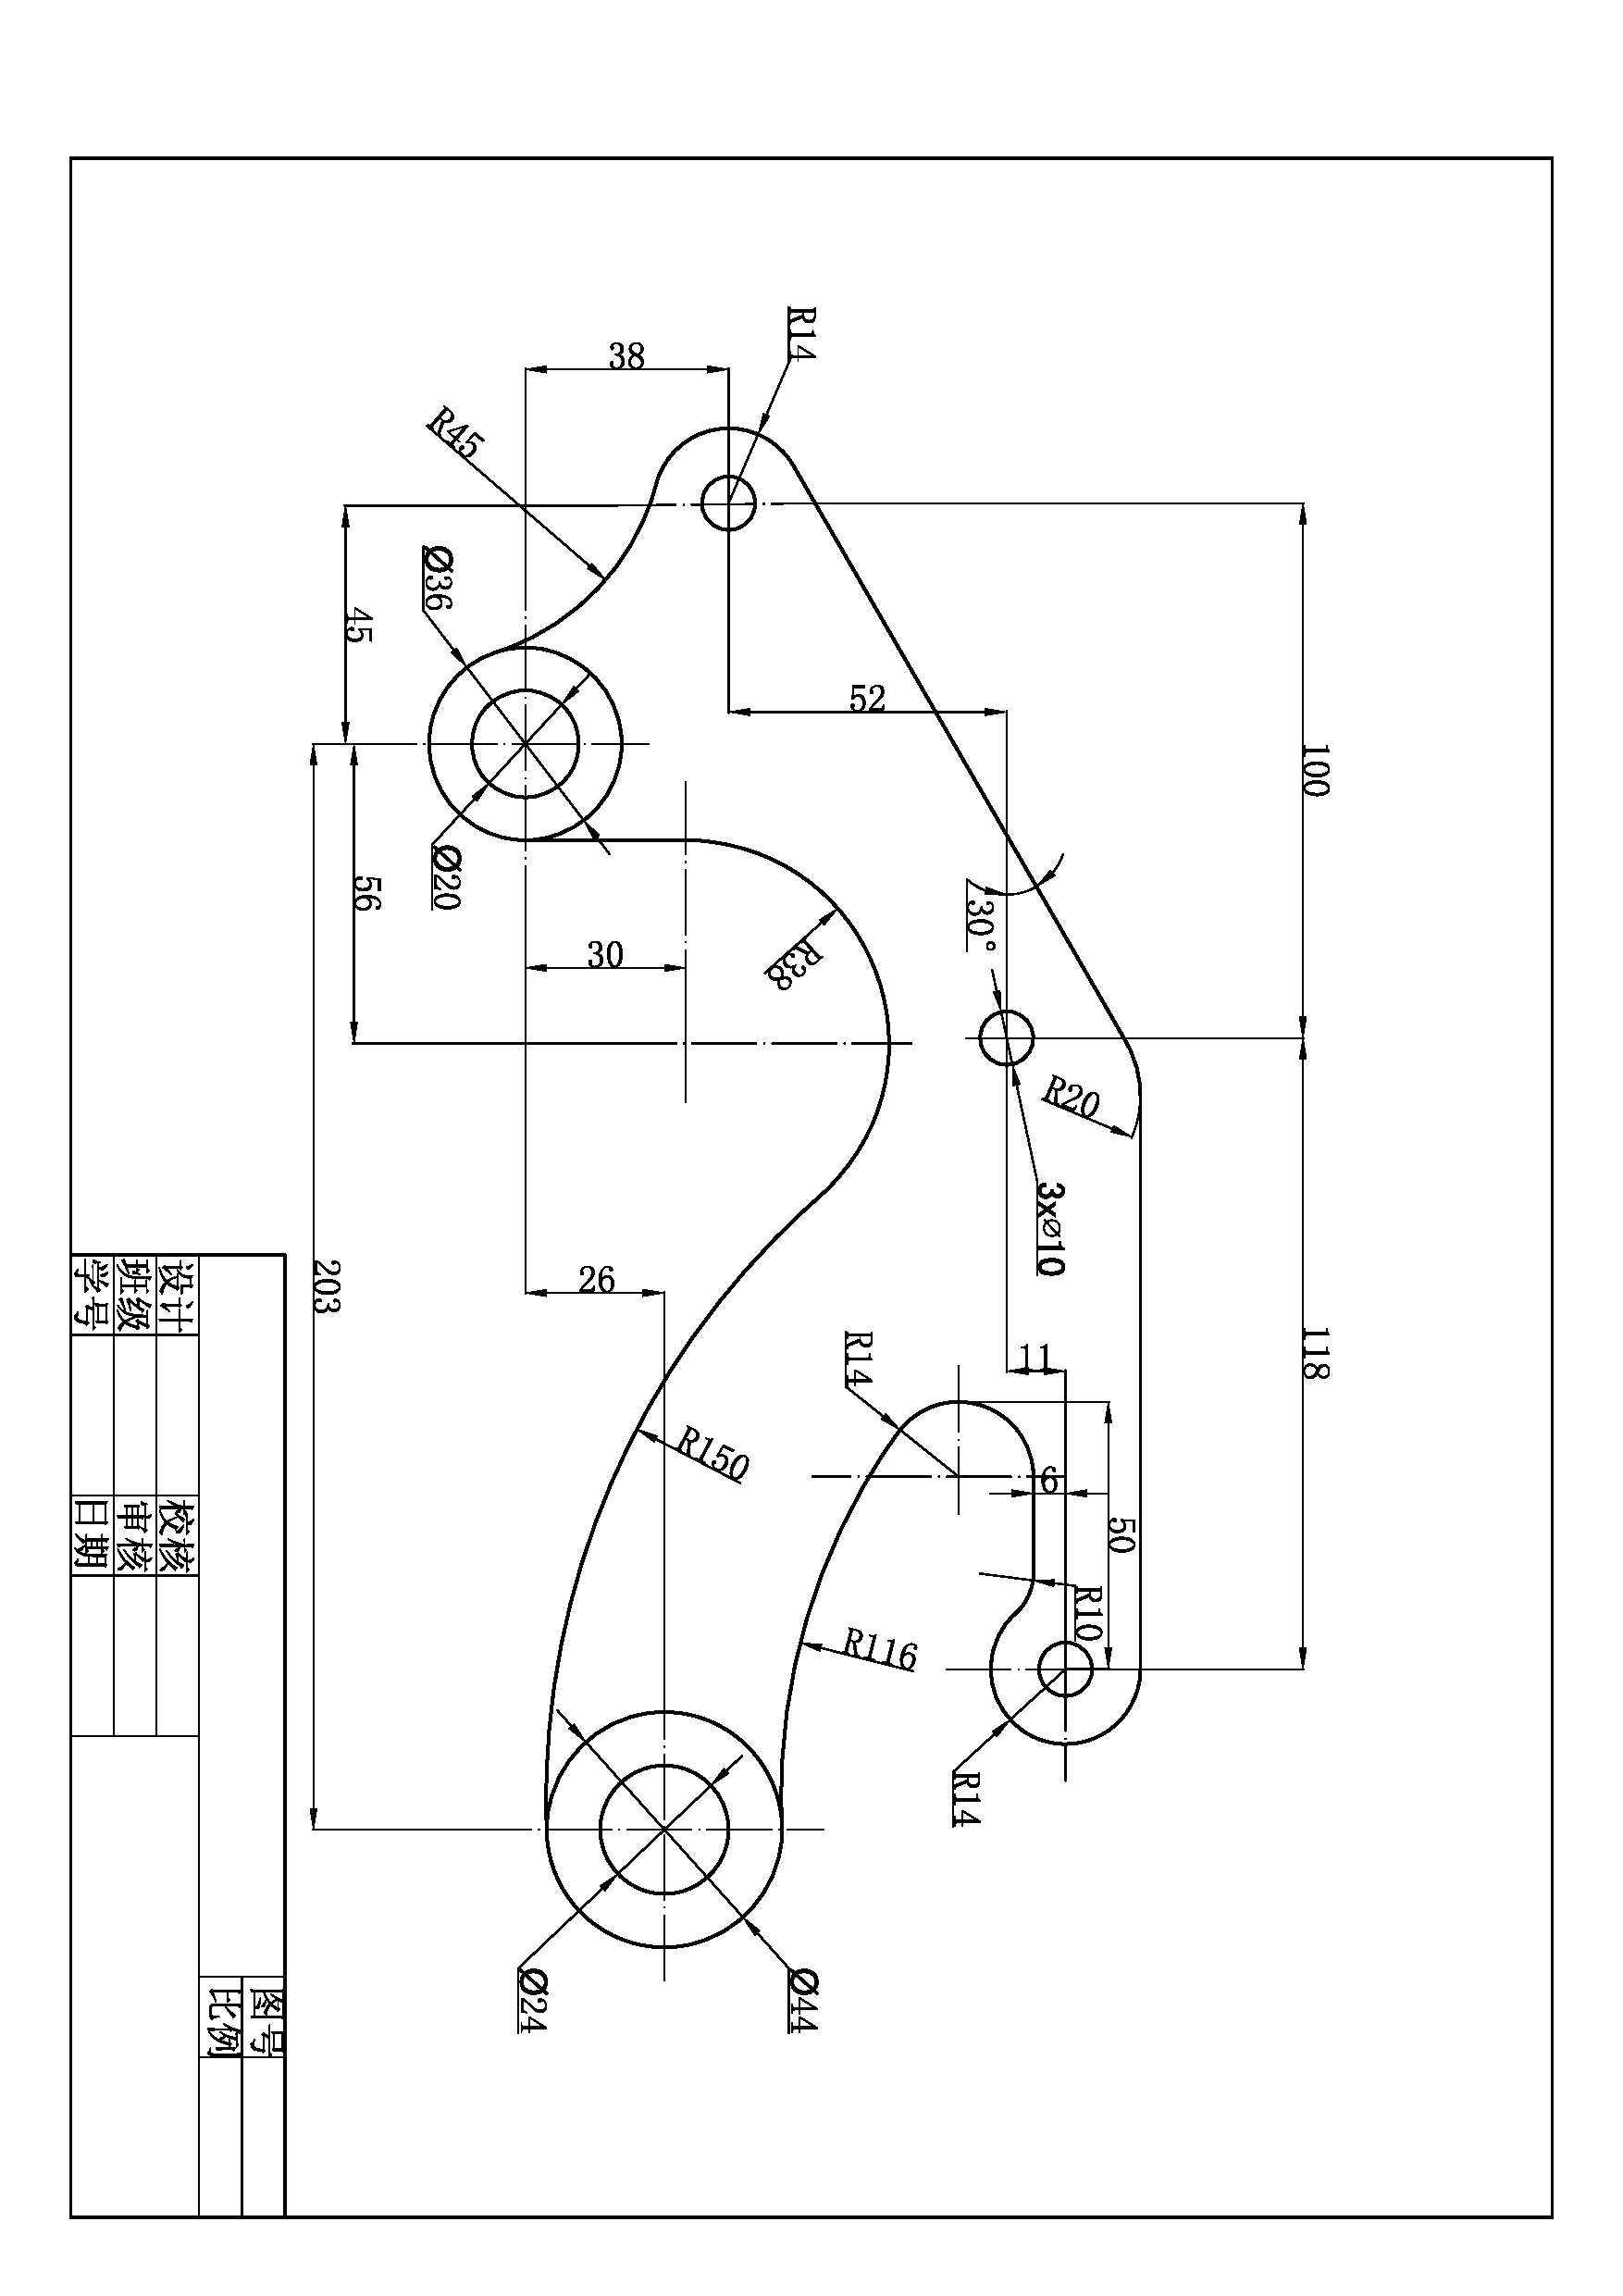
\includegraphics[scale=0.45,angle=90]{shu1.pdf}
\caption{项目一示例}\label{fig:shangmu1}
\end{figure}
\end{landscape}
\indent
%\newpage

\section{平面几何图(一)}\label{sec:gongzhi}

{\bfseries 知识目标}
\begin{itemize}
\item 掌握绝对坐标、相对坐标和极轴坐标的概念
\item 掌握limits命令的使用方法
\item 掌握point、line命令的使用方法
\item 了解国家制图标准中图幅的标准及与limits命令之间的关系
\end{itemize}

{\bfseries 技能目标}
\begin{itemize}
\item 能够完成工字图样的绘制
\end{itemize}

本任务以绘制图\ref{fig:shangmu1-1}所示的工字图样为目标,主要是为了帮助读者掌握Auto\-CAD 图形绘制过程中最重要的概念---坐标。坐标是AutoCAD精确绘的基础,对图形对象的精确定位起至关重要的作用。通过完成该任务来理解AutoCAD中图形的关键点的坐标描述方法,以及各种坐标表述方式的应用情景。其次是为了让读者掌握line命令的基本用法。
\enlargethispage{10pt}
\noindent
\begin{figure}[htbp]
\centering
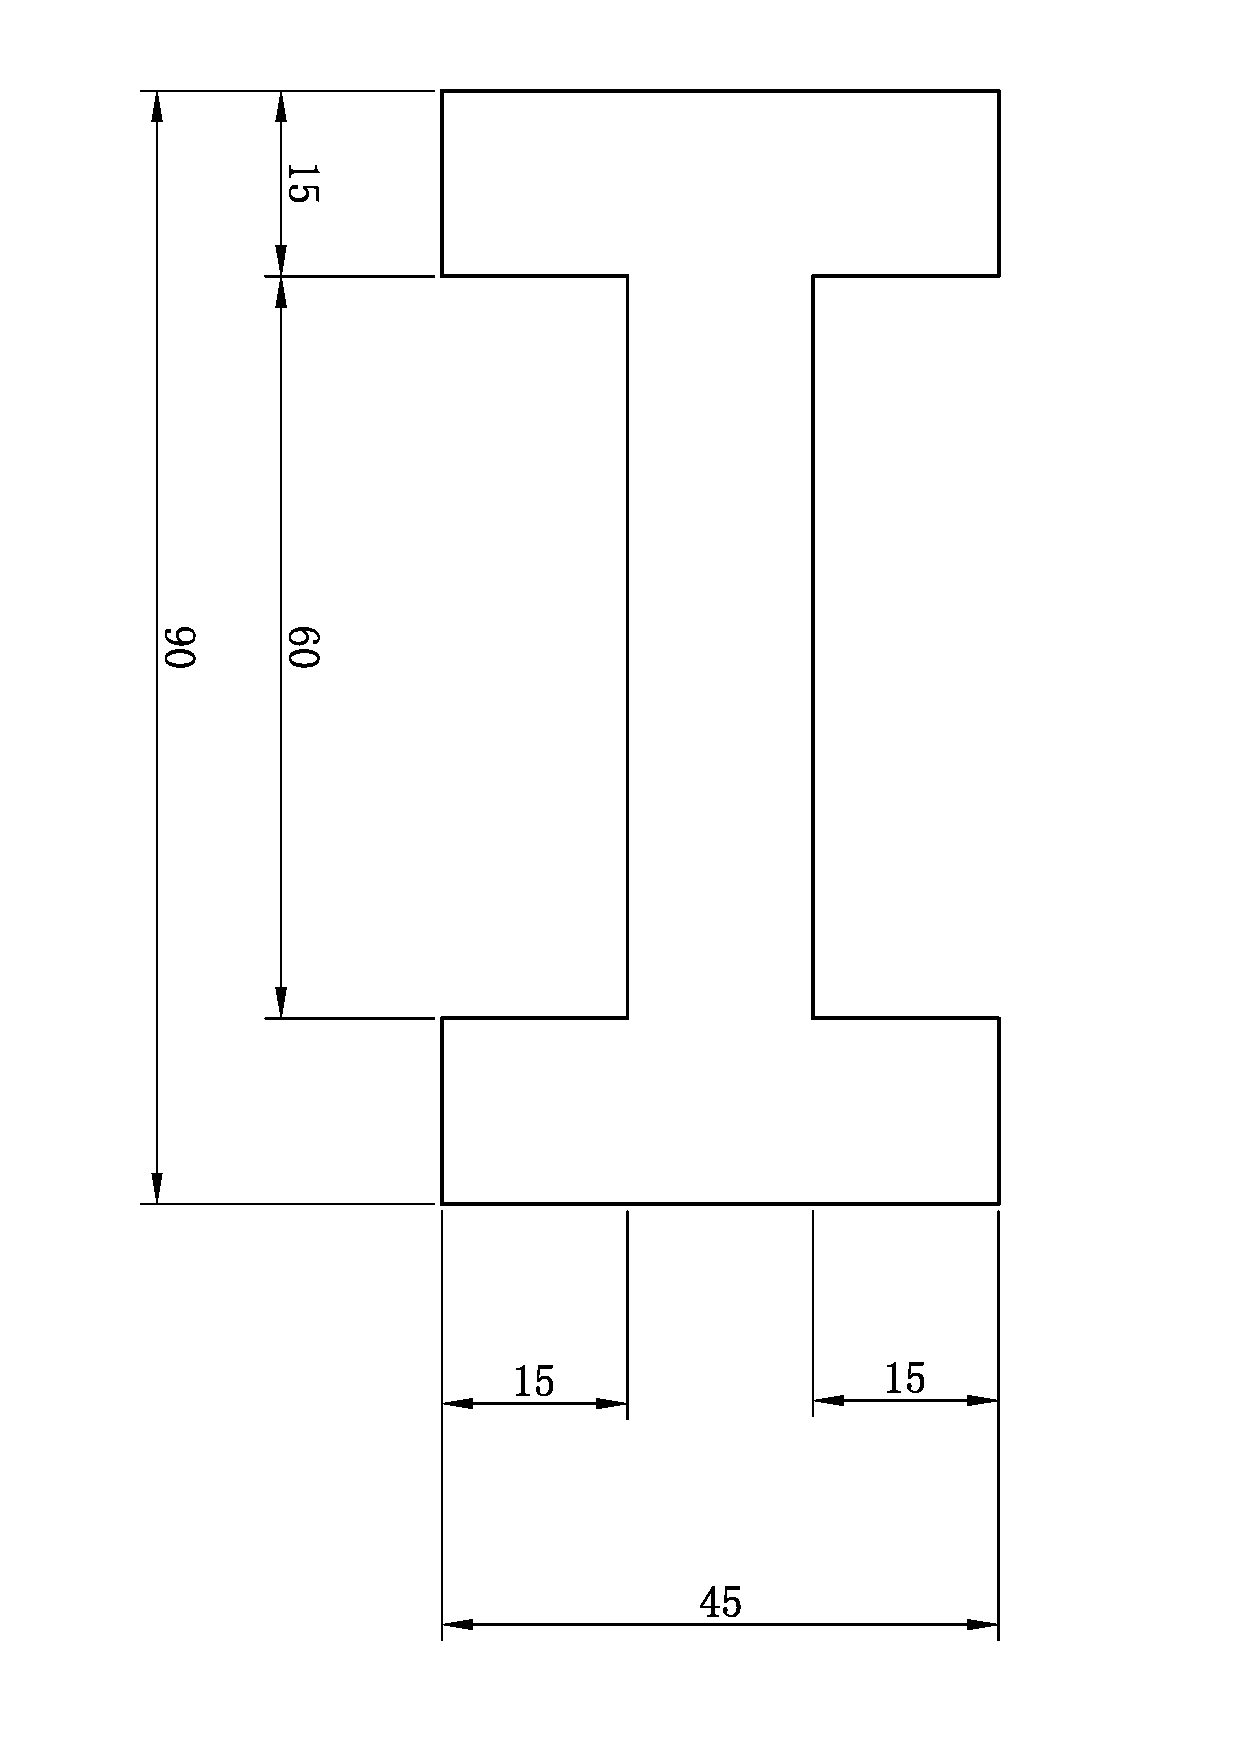
\includegraphics[scale=0.4,angle=90]{gongzi.pdf}
\caption{工字图样}\label{fig:shangmu1-1}
\end{figure}
\indent

\subsection{绘制图样}
\subsubsection{设置图形界限LIMITS}
AutoCAD中的绘图区域是无限大的,可以在绘图区的任何地方绘图。为一方便打印,一般需要设置一个绘图区域用来限制绘图的区域,不至于将图形绘制来区域之外。要实现此功能,用户使用“图形界限”命令进行设置。

在命令提示区输入limits 以执行“图形界限”命令。
\noindent
命令:  LIMITS\\
重新设置模型空间界限:\\
指定左下角点或 [开(ON)/关(OFF)] $<$0.0000,0.0000$>$:\\
指定右上角点 $<$420.0000,297.0000$>$: 297,210\\
\indent
LIMITS命令中【开(ON)】表示打开界限检查,此时不能够在图形界限以外输入点来创建图形对象。【关(OFF)】表示关闭界限检查,此时能够在图形界限以外输入图形对象。

\subsubsection{图形缩放显示ZOOM}
由于图\ref{fig:shangmu1-1}的尺寸比较小,为了便于观察绘图结果,我们需要先使用ZOOM命令先将图形显示区域缩放到图形界限范围。

\noindent
命令: ZOOM\\
指定窗口的角点,输入比例因子 (nX 或 nXP),或者
[全部(A)/中心(C)/动态(D)/范围(E)/上一个(P)/比例(S)/窗口(W)/对象(O)] $<$实时$>$: a
\indent

ZOOM命令中各个选项的含义如下:
\begin{itemize}
\item 全部(A):在平面图形中,缩放到整个图形界限
\item 中心(C):缩放显示由中心点和缩放比例(或高度)所定义的窗口
\item 动态(D):执行此选项,会出现一个视图框,通过调整视图框的大小,调整显示图形的大小
\item 范围(E):最大限度的显示所有图形
\item 上一个(P):回到上一次缩放
\item 比例(s):按输入比例值进行缩放
\item 窗口(W):最大限度地显示框选的图形
\item 对象(O):最大限度地显示选择的对象
\end{itemize}
\subsubsection{绘制图形}
绘制图\ref{fig:shangmu1-1}需要使用AutoCAD中的line命令。

\noindent
命令: line 指定第一点: 0,0\\
指定下一点或 [放弃(U)]: @0,45\\
指定下一点或 [放弃(U)]: @15,0\\
指定下一点或 [闭合(C)/放弃(U)]: @-15$<$90\\
指定下一点或 [闭合(C)/放弃(U)]: @60$<$0\\
指定下一点或 [闭合(C)/放弃(U)]: @15$<$90\\
指定下一点或 [闭合(C)/放弃(U)]: @15$<$0\\
指定下一点或 [闭合(C)/放弃(U)]: @45$<$-90\\
指定下一点或 [闭合(C)/放弃(U)]: @15$<$180\\
指定下一点或 [闭合(C)/放弃(U)]: @15$<$90\\
指定下一点或 [闭合(C)/放弃(U)]: @-60$<$0\\
指定下一点或 [闭合(C)/放弃(U)]: @-15$<$90\\
指定下一点或 [闭合(C)/放弃(U)]: c

\indent
line命令中【放弃(U)】表示删除直线序列中最近绘制的线段。【闭合(C)】表示当以第一条线段的起点和最后一线段的端点,形成一个闭合的线段环。注意到上面的提示序列,只有线段数大于等两条时该选项才可以使用。

\zhishi{坐标理论}
坐标是精确定位AutoCAD对象的基础,在\ref{sec:gongzhi}中使用了$(x,y)$、$(@x,y)$ 和 $(@$距离$<$角度$)$三种形式来表示式字图形的各个牲点位置。此种形式即为Auto\-CAD 的坐标表示方式。
\subsection{卡笛尔坐标系}
卡笛尔坐标系即为直角坐标系,是用通过原点$O(0,0)$的两个相互垂直的坐标轴$X$和$Y$来表示绘图区域。图中的每一个点均表示为$(x,y)$的形式,如图\ref{fig:zuobiao1}所示。
\begin{figure}[htbp]
\centering
\begin{floatrow}
\ffigbox{\caption{坐标表示}\label{fig:zuobiao1}}{
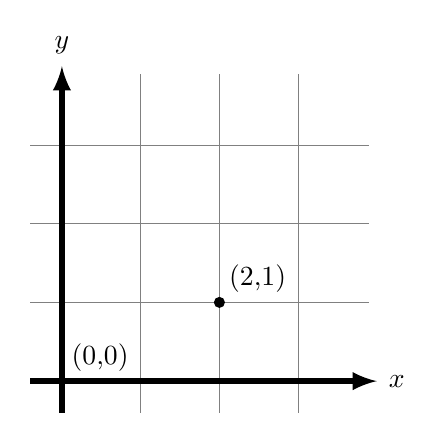
\begin{tikzpicture}
\draw[help lines,step=1cm,very thin](-0.4cm,-0.4cm)grid(3.9cm,3.9cm);
\draw[->,line width=0.7mm](-0.4cm,0)--(4cm,0)node[right]{$x$};
\draw[->,line width=0.7mm](0,-0.4cm)--(0,4cm)node[above]{$y$};
\draw (0,0)node[above right]{(0,0)};
\fill (2cm,1cm)node[above right]{(2,1)}circle(2pt);
\end{tikzpicture}}
\ffigbox{\caption{极坐标表示}\label{fig:jizuobiao1}}{
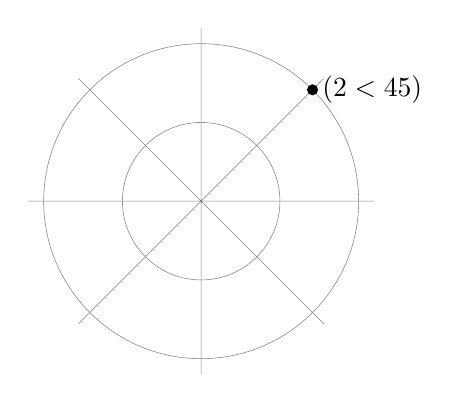
\begin{tikzpicture}
\draw[help lines,very thin](-2.2cm,0)--(2.2cm,0)(0,-2.2cm)--(0,2.2cm)(45:2.2cm)--(225:2.2cm)(135:2.2cm)--(-45:2.2cm);
\draw[help lines,very thin](0,0)circle(1cm)circle(2cm);
\fill (45:2cm)node[right]{$(2<45\degree)$}circle(2pt);
\end{tikzpicture}
}
\end{floatrow}
\end{figure}
\subsection{极坐标系}
极坐标系是一个二维坐标系统,它用一段相对于中心点的距离和一个夹角来表示坐标区域中的点,其坐形式为$(\rho,\theta)$,如图\ref{fig:jizuobiao1}所示。其中$\rho$表示距离,永远取正值,$\theta$表示角度,取值范围为$0-360\degree$。
\subsection{绝坐标和相对坐标}
绝对坐标是以当前坐标原点为基点进行参照所获得的坐标值。如$(3,5)$,$(4<45\degree)$。

相对坐标是以前面输入的坐标点为参照所获得的坐标值,表示方法是在坐标值前面加一个“@”符号。例如,相对直角坐标表示为$(@5,4)$,相对极坐标表示为$(@5<35)$。

例如,绘制一条两个端点分别为$(3,5)$和$(6,9)$的直线。调用line命令:

\noindent
命令: line 指定第一点: 3,5\\
指定下一点或 [放弃(U)]:\\
用绝对坐标方式输入,$(6,9)$就可以绘出直线。\\
用相对坐标方式输入,可知$(6,9)$相对于$(3,5)$的$X$轴增量为3,$Y$轴增量为4,故输入相对坐标$(@3,4)$也可以绘出直线。

\indent
但是,从AutoCAD的实际绘图过程来看,多种坐标输入方式配合使用会使整个绘图过程更加灵活和方便,再配合目标捕捉和夹点编辑等方式,则使绘图更精确、更快捷。
\zhishi{图纸幅面及格式}
\subsection{图纸幅面}
“图形界限”中我们所设置的297$\times $210的尺寸就是国家标准中的A4图纸幅面。国家标准《技术制图》中规定幅面的尺寸是为了方便绘制、使用和保管图样。因此,在绘制图样时,应优先采用表\ref{tab:tufubiao1}中规定的尺寸,必要时允许先用规定的加长幅面,加长幅面的尺寸由基本幅面短边的成整数倍增加后得出,如图\ref{fig:tufujiachang}所示。其中粗实细部分为基本幅面。加长后幅面记作:基本幅面代号$\times $倍数。如$A3\times 3$,表示按A3图幅短边加长为297mm的3倍,即加长后图纸尺寸为$420mm\times 891mm$。
%\suppressfloats[t]
\begin{table}[htbp]
\caption{图纸幅面及周边尺寸}\label{tab:tufubiao1}
\begin{tabular}{*{6}{c|}c}
\hline
\multicolumn{2}{c|}{幅面代号}&A0&A1&A2&A3&A4\\ \hline
\multicolumn{2}{c|}{尺寸 $B\times L$}&$841\times 1189$&$594\times 841$&$420\times 594$&$297\times 420$&$210\times 297$\\ \hline
\multirow{3}*{图框}&a&\multicolumn{5}{|c}{25}\\ \cline{2-7}
&c&\multicolumn{3}{|c}{10}&\multicolumn{2}{|c}{5}\\ \cline{2-7}
&e&\multicolumn{2}{|c}{20}&\multicolumn{3}{|c}{10}\\
\hline
\end{tabular}
\end{table}

\begin{figure}[htbp]
\centering
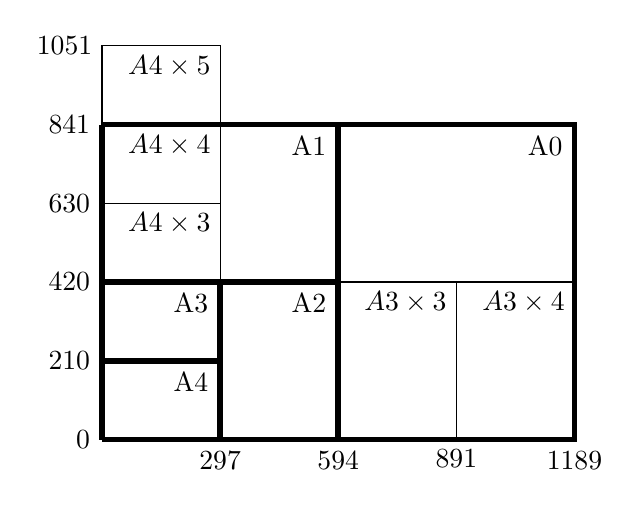
\begin{tikzpicture}
\draw[line width=0.7mm] (0,0)node[left]{0}--(0,1cm)node[left]{210}--(0,2cm)node[left]{420}--(0,3cm)node[left]{630}--(0,4cm)node[left]{841};
\draw(0,4cm)--(0,5cm)node[left]{1051}--(1.5cm,5cm)node[below left]{$A4\times 5$}--(1.5cm,2cm);
\draw[line width=0.7mm](0,1cm)--(1.5cm,1cm)node[below left]{A4}(0,2cm)--(1.5cm,2cm)node[below left]{A3}--(1.5cm,0)node[below]{297};
\draw(0,3cm)--(1.5cm,3cm)node[below left]{$A4\times 3$};
\draw[line width=0.7mm](0,4cm)--(3cm,4cm)node[below left]{A1}--(3cm,0)node[below]{594}(1.5cm,2cm)--(3cm,2cm)node[below left]{A2};
\draw[line width=0.7mm](3cm,4cm)--(6cm,4cm)node[below left]{A0}--(6cm,0)node[below]{1189}--(0,0);
\draw(3cm,2cm)--(4.5cm,2cm)node[below left]{$A3\times 3$}--(6cm,2cm)node[below left]{$A3\times 4$}(4.5cm,2cm)--(4.5cm,0)node[below]{891};
\draw(1.5cm,4cm)node[below left]{$A4\times 4$};
\end{tikzpicture}
\caption{图纸幅面及加长边} \label{fig:tufujiachang}
\end{figure}

从表\ref{tab:tufubiao1}中可以看出幅面之间的关系为:将A0图纸的长边对折后得到两张A1图纸,将A1图纸的长边对折后得到两纸A2图纸,以此类推。

\subsection{标题栏}
每张图样上必须画出标题栏,标题栏位于图样的右下角,与看图的方向一致。

标题栏分为更必区、签字区、名称及代号区和其他区,如图\ref{fig:biaotilan}所示。
\tikzset{
>=latex,
center lines/.style={dash pattern=on 20pt off 3pt on 2pt off 3pt},
importance lines/.style={line width=1pt}
}
\noindent
\begin{figure}[htbp]
\begin{tikzpicture}[scale=0.65]
\draw[line width=0.7mm](0,0)rectangle(180mm,56mm);
\draw(0,7mm)--(12mm,7mm)--(40mm,7mm)--++(40mm,0);
\draw(6mm,3.5mm)node{\tiny 工艺};
\draw(46mm,3.5mm)node{\tiny 批准};
\draw(0,14mm)--++(80mm,0);
\draw(6mm,10.5mm)node{\tiny 审核};
\draw(0,21mm)--++(12mm,0)--++(12mm,0)--++(16mm,0)--++(12mm,0)--++(12mm,0)--++(16mm,0);
\draw(6mm,24.5mm)node{\tiny设计};
\draw(18mm,24.5mm)node{\tiny(签名)};
\draw(32mm,24.5mm)node{\tiny(年月日)};
\draw(46mm,24.5mm)node{\tiny标准化};
\draw(58mm,24.5mm)node{\tiny签名};
\draw(72mm,24.5mm)node{\tiny(年月日)};
\draw(12mm,0)--++(0,28mm)(24mm,0)--++(0,28mm)(40mm,0)--++(0,28mm)(52mm,0)--++(0,28mm)(64mm,0)--++(0,28mm)(80mm,0)--++(0,28mm);
\draw(0,28mm)--++(10mm,0)--++(10mm,0)--++(16mm,0)--++(16mm,0)--++(12mm,0)--++(16mm,0);
\draw(5mm,31.5mm)node{\tiny 标记};
\draw(15mm,31.5mm)node{\tiny 处数};
\draw(28mm,31.5mm)node{\tiny 分区};
\draw(44mm,31.5mm)node{\tiny 更改文件号};
\draw(56mm,31.5mm)node{\tiny 签名};
\draw(72mm,31.5mm)node{\tiny 年月日};
\draw(0,35mm)--++(80mm,0)(0,42mm)--++(80mm,0)(0,49mm)--++(80mm,0);
\draw(10mm,28mm)--++(0,28mm)(20mm,28mm)--++(0,28mm)(36mm,28mm)--++(0,28mm)(52mm,28mm)--++(0,28mm)(64mm,28mm)--++(0,28mm)(80mm,28mm)--++(0,28mm);
\draw(80mm,9mm)--++(50mm,0);
\draw(105mm,4.5mm)node{\tiny 共\quad张\quad第\quad张};
\draw(80mm,18mm)--++(26mm,0)--++(12mm,0)--++(12mm,0);
\draw(93mm,23mm)node{\tiny 阶段标记};
\draw(112mm,23mm)node{\tiny 重量};
\draw(124mm,23mm)node{\tiny 比例};
\draw(86.5mm,9mm)--++(0,9mm)(93mm,9mm)--++(0,9mm)(99.5mm,9mm)--++(0,9mm)(106mm,9mm)--++(0,18mm)(118mm,9mm)--++(0,18mm);
\draw(80mm,28mm)--++(50mm,0);
\draw(130mm,0)--++(0,56mm);
\draw(130mm,18mm)--++(50mm,0)(130mm,38mm)--++(50mm,0);
\draw (155mm,9mm)node{\tiny(图样代号)};
\draw(155mm,28mm)node{\tiny(图样名称)};
\draw(155mm,48mm)node{\tiny(单位名称)};
\draw(105mm,48mm)node{\tiny(材料标记)};
\draw[<->](99.5mm,12mm)--(106mm,12mm)node[midway,above]{\tiny 6.5};
\draw(-14mm,0)--(0,0)(-7mm,7mm)--(0,7mm)(-14mm,56mm)--(0,56mm);
\draw[<->](-5mm,0)--(-5mm,7mm)node[midway,above,rotate=90]{\tiny 7};
\draw[<->](-13mm,0)--(-13mm,56mm)node[midway,above,rotate=90]{\tiny $8\times 7(56)$};
\draw(130mm,9mm)--++(9mm,0)(130mm,28mm)--++(9mm,0);
\draw[<->](137mm,0)--++(0,9mm)node[midway,above,rotate=90]{\tiny 9};
\draw[<->](137mm,9mm)--++(0,9mm)node[midway,above,rotate=90]{\tiny 9};
\draw[<->](137mm,18mm)--++(0,10mm)node[midway,above,rotate=90]{\tiny 10};
\draw(180mm,0)--++(9mm,0)(180mm,18mm)--++(9mm,0)(180mm,38mm)--++(9mm,0);
\draw[<->](187mm,0)--++(0,18mm)node[midway,above,rotate=90]{\tiny 18};
\draw[<->](187mm,18mm)--++(0,20mm)node[midway,above,rotate=90]{\tiny 20};
\draw(0,-9mm)--++(0,9mm)(12mm,-9mm)--++(0,9mm)(24mm,-9mm)--++(0,9mm)(40mm,-9mm)--++(0,9mm)(52mm,-9mm)--++(0,9mm)(64mm,-9mm)--++(0,9mm)(80mm,-9mm)--++(0,9mm)(130mm,-9mm)--++(0,9mm);
\draw[<->](0,-7mm)--++(12mm,0)node[midway,above]{\tiny 12};
\draw[<->](12mm,-7mm)--++(12mm,0)node[midway,above]{\tiny 12};
\draw[<->](24mm,-7mm)--++(16mm,0)node[midway,above]{\tiny 16};
\draw[<->](40mm,-7mm)--++(12mm,0)node[midway,above]{\tiny 12};
\draw[<->](52mm,-7mm)--++(12mm,0)node[midway,above]{\tiny 12};
\draw[<->](64mm,-7mm)--++(16mm,0)node[midway,above]{\tiny 16};
\draw[<->](80mm,-7mm)--++(50mm,0)node[midway,above]{\tiny 50};
\draw(0,-18mm)--(0,0)(180mm,-18mm)--(180mm,0);
\draw[<->](0,-16mm)--(180mm,-16mm)node[midway,above]{\tiny 180};
\draw(0,56mm)--++(0,7mm)(10mm,56mm)--++(0,7mm)(20mm,56mm)--++(0,7mm)(36mm,56mm)--++(0,7mm)(52mm,56mm)--++(0,7mm)(64mm,56mm)--++(0,7mm)(80mm,56mm)--++(0,7mm);
\draw[<->](0,61mm)--++(10mm,0)node[midway,above]{\tiny 10};
\draw[<->](10mm,61mm)--++(10mm,0)node[midway,above]{\tiny 10};
\draw[<->](20mm,61mm)--++(16mm,0)node[midway,above]{\tiny 16};
\draw[<->](36mm,61mm)--++(16mm,0)node[midway,above]{\tiny 16};
\draw[<->](52mm,61mm)--++(12mm,0)node[midway,above]{\tiny 12};
\draw[<->](64mm,61mm)--++(16mm,0)node[midway,above]{\tiny 16};
\draw(106mm,28mm)--++(0,7mm)(118mm,28mm)--++(0,7mm);
\draw[<->](80mm,33mm)--++(26mm,0)node[midway,above]{\tiny $4\times 6.5(26)$};
\draw[<->](106mm,33mm)--++(12mm,0)node[midway,above]{\tiny 12};
\draw[<->](118mm,33mm)--++(12mm,0)node[midway,above]{\tiny 12};
\end{tikzpicture}
\caption{标题栏格式及尺寸}\label{fig:biaotilan}
\end{figure}
\indent

\subsection{图框格式}
图框格式分为留装订边和不留装订边两种,其装订边尺寸如表\ref{tab:tufubiao1}所示。图\ref{fig:zhuangding}所示为采用A4幅面竖装和A3幅面横装时,留装订边和不留装订边的图框格式。
\noindent
\tikzset{
>=latex,
center lines/.style={dash pattern=on 20pt off 3pt on 2pt off 3pt},
importance lines/.style={line width=1pt}
}
\begin{figure}[htbp]
\centering
\subfloat[留装订边格式]{
\begin{tikzpicture}
\draw(0,0)rectangle(4cm,5cm);
\draw[line width=0.7mm](0.5cm,0.25cm)rectangle(3.75cm,4.75cm)(1.5cm,0.25cm)--(1.5cm,1cm)--(3.75cm,1cm)node[midway,below]{标题栏};
\draw(-0.7cm,0)--(0,0)(-0.7cm,5cm)--(0cm,5cm);
\draw[<->](-0.5cm,0)--(-0.5cm,5cm)node[midway,above,rotate=90]{$L$};
\draw(0,-0.7cm)--(0,0)(4cm,-0.7cm)--(4cm,0);
\draw[<->](0,-0.5cm)--(4cm,-0.5cm)node[midway,above]{$B$};
\draw[->](1cm,-0.45cm)--(1cm,0);
\draw[->](1cm,0.65cm)--(1cm,0.25cm)node[midway,above,rotate=90]{$c$};
\draw(1cm,0)--(1cm,0.25cm);
\draw[->](-0.4cm,2cm)--(0,2cm);
\draw[->](0.9cm,2cm)--(0.5cm,2cm);
\draw(0,2cm)--(0.5cm,2cm)node[midway,above]{$a$};
\draw[->](2cm,5cm)--(2cm,4.35cm)--(2cm,4.75cm);
\draw[->](2cm,5.45cm)--(2cm,5cm)node[midway,above,rotate=90]{$c$};
\draw[->](4cm,2.5cm)--(3.3cm,2.5cm)--(3.75cm,2.5cm);
\draw[->](4.45cm,2.5cm)--(4cm,2.5cm)node[midway,above]{$c$};

\begin{scope}[xshift=5.5cm]
\draw(0,0)rectangle(7cm,5cm);
\draw[line width=0.7mm](0.5cm,0.25cm)rectangle(6.75cm,4.75cm)(4.5cm,0.25cm)--(4.5cm,1cm)--(6.75cm,1cm)node[midway,below]{标题栏};
\draw(-0.7cm,0)--(0,0)(-0.7cm,5cm)--(0cm,5cm);
\draw[<->](-0.5cm,0)--(-0.5cm,5cm)node[midway,above,rotate=90]{$B$};
\draw(0,-0.7cm)--(0,0)(7cm,-0.7cm)--(7cm,0);
\draw[<->](0,-0.5cm)--(7cm,-0.5cm)node[midway,above]{$L$};
\draw[->](3cm,-0.45cm)--(3cm,0);
\draw[->](3cm,0.65cm)--(3cm,0.25cm)node[midway,above,rotate=90]{$c$};
\draw(3cm,0)--(3cm,0.25cm);
\draw[->](-0.4cm,2cm)--(0,2cm);
\draw[->](0.9cm,2cm)--(0.5cm,2cm);
\draw(0,2cm)--(0.5cm,2cm)node[midway,above]{$a$};
\draw[->](3.5cm,5cm)--(3.5cm,4.35cm)--(3.5cm,4.75cm);
\draw[->](3.5cm,5.45cm)--(3.5cm,5cm)node[midway,above,rotate=90]{$c$};
\draw[->](7cm,2.5cm)--(6.3cm,2.5cm)--(6.75cm,2.5cm);
\draw[->](7.45cm,2.5cm)--(7cm,2.5cm)node[midway,above]{$c$};
\end{scope}
\end{tikzpicture}}

\subfloat[不留装订边格式]{
\begin{tikzpicture}
\draw(0,0)rectangle(4cm,5cm);
\draw[line width=0.7mm](0.25cm,0.25cm)rectangle(3.75cm,4.75cm)(1.5cm,0.25cm)--(1.5cm,1cm)--(3.75cm,1cm)node[midway,below]{标题栏};
\draw(-0.7cm,0)--(0,0)(-0.7cm,5cm)--(0cm,5cm);
\draw[<->](-0.5cm,0)--(-0.5cm,5cm)node[midway,above,rotate=90]{$L$};
\draw(0,-0.7cm)--(0,0)(4cm,-0.7cm)--(4cm,0);
\draw[<->](0,-0.5cm)--(4cm,-0.5cm)node[midway,above]{$B$};
\draw[->](1cm,-0.45cm)--(1cm,0);
\draw[->](1cm,0.65cm)--(1cm,0.25cm)node[midway,above,rotate=90]{$c$};
\draw(1cm,0)--(1cm,0.25cm);
\draw[->](-0.4cm,2cm)--(0,2cm);
\draw[->](0.65cm,2cm)--(0.25cm,2cm)node[midway,above]{$c$};
\draw(0,2cm)--(0.25cm,2cm);
\draw[->](2cm,5cm)--(2cm,4.35cm)--(2cm,4.75cm);
\draw[->](2cm,5.45cm)--(2cm,5cm)node[midway,above,rotate=90]{$c$};
\draw[->](4cm,2.5cm)--(3.3cm,2.5cm)--(3.75cm,2.5cm);
\draw[->](4.45cm,2.5cm)--(4cm,2.5cm)node[midway,above]{$c$};

\begin{scope}[xshift=5.5cm]
\draw(0,0)rectangle(7cm,5cm);
\draw[line width=0.7mm](0.25cm,0.25cm)rectangle(6.75cm,4.75cm)(4.5cm,0.25cm)--(4.5cm,1cm)--(6.75cm,1cm)node[midway,below]{标题栏};
\draw(-0.7cm,0)--(0,0)(-0.7cm,5cm)--(0cm,5cm);
\draw[<->](-0.5cm,0)--(-0.5cm,5cm)node[midway,above,rotate=90]{$B$};
\draw(0,-0.7cm)--(0,0)(7cm,-0.7cm)--(7cm,0);
\draw[<->](0,-0.5cm)--(7cm,-0.5cm)node[midway,above]{$L$};
\draw[->](3cm,-0.45cm)--(3cm,0);
\draw[->](3cm,0.65cm)--(3cm,0.25cm)node[midway,above,rotate=90]{$c$};
\draw(3cm,0)--(3cm,0.25cm);
\draw[->](-0.4cm,2cm)--(0,2cm);
\draw[->](0.65cm,2cm)--(0.25cm,2cm)node[midway,above]{$c$};
\draw(0,2cm)--(0.25cm,2cm);
\draw[->](3.5cm,5cm)--(3.5cm,4.35cm)--(3.5cm,4.75cm);
\draw[->](3.5cm,5.45cm)--(3.5cm,5cm)node[midway,above,rotate=90]{$c$};
\draw[->](7cm,2.5cm)--(6.3cm,2.5cm)--(6.75cm,2.5cm);
\draw[->](7.45cm,2.5cm)--(7cm,2.5cm)node[midway,above]{$c$};
\end{scope}
\end{tikzpicture}}
\caption{图框格式}\label{fig:zhuangding}
\end{figure}
\indent
\clearpage
\section{平面几何作图(二)}

{\bfseries 知识目标}
\begin{itemize}
\item 掌握layger命令和图层定义和使用方法
\item 掌握xline命令的使用方法
\item 掌握circle命令的使用方法
\item 掌握多边形命令的使用方法
\item 掌握图形阵列命令的使用方法
\end{itemize}

{\bfseries 技能目标}
\begin{itemize}
\item 能够完成简单图样的绘制
\item 具备用AutoCAD图层管理图线的能力
\end{itemize}

\noindent
\begin{figure}[htbp]
\centering
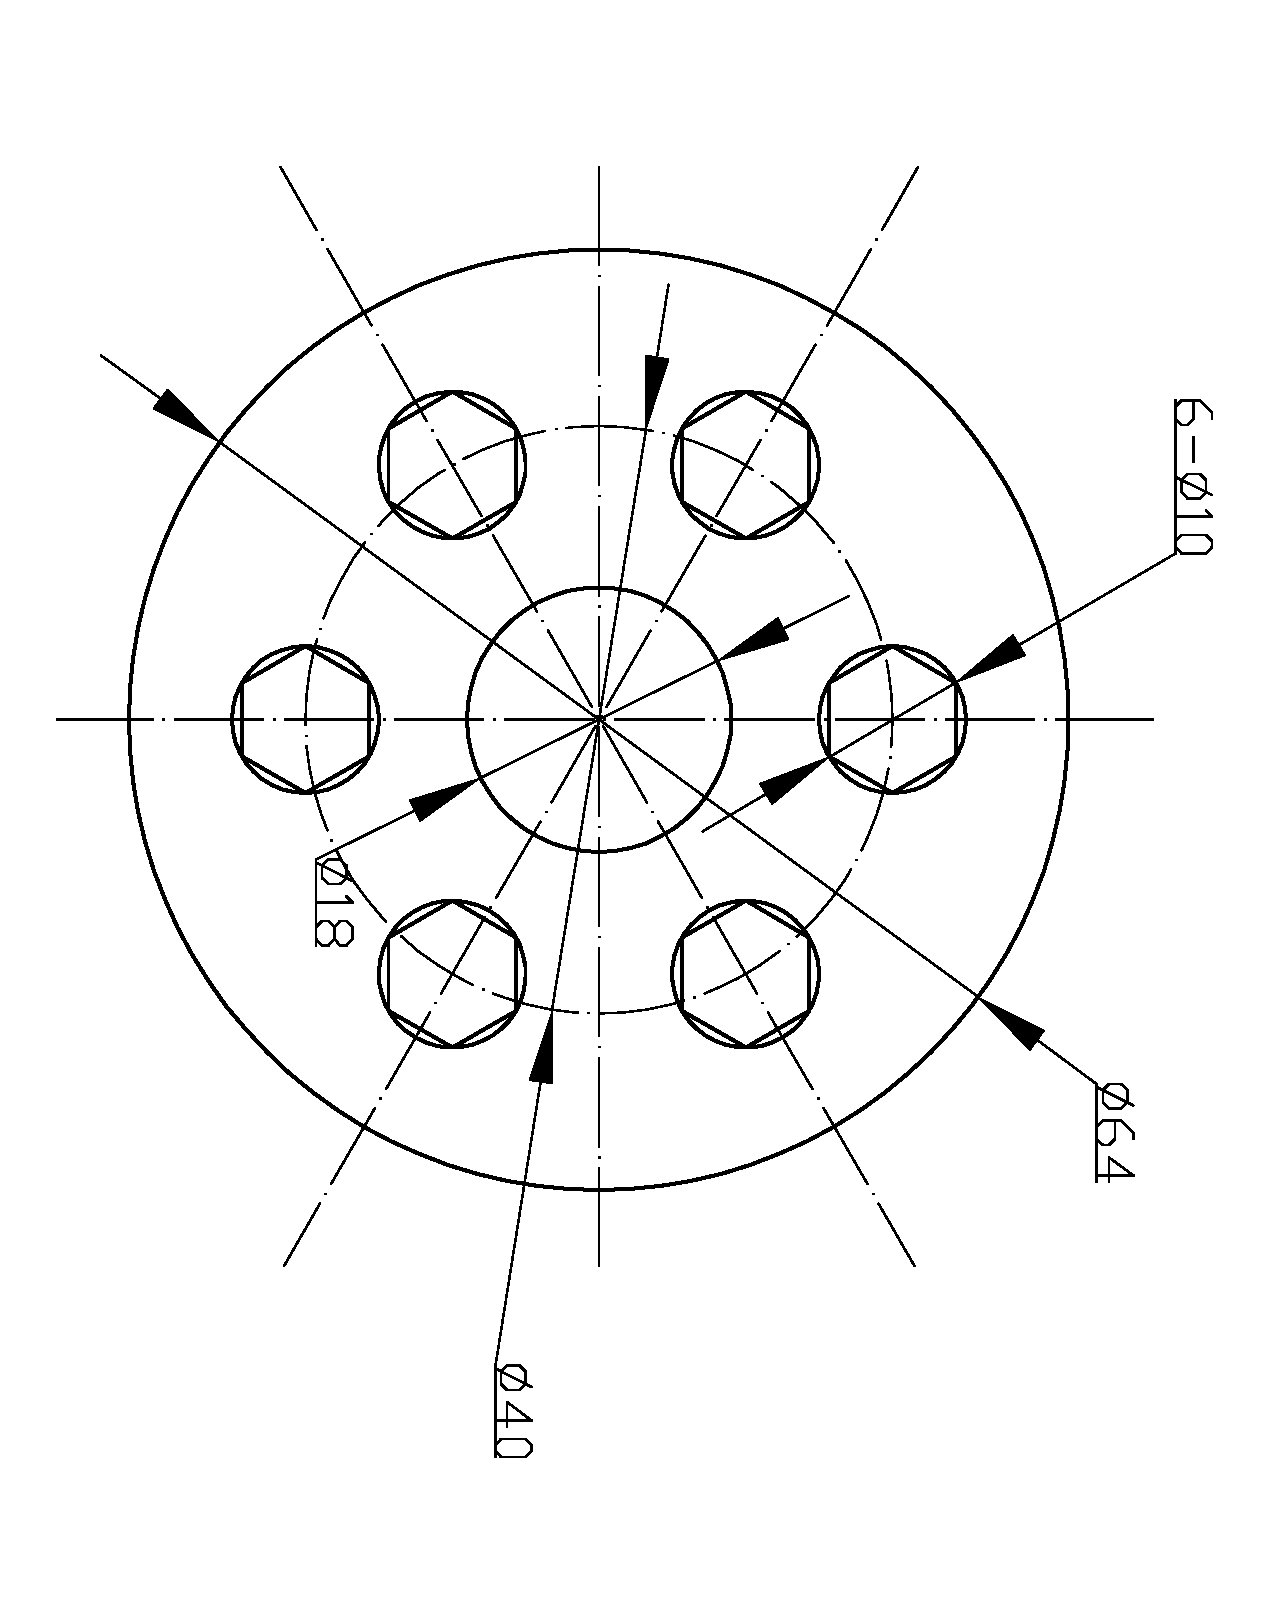
\includegraphics[scale=0.45,angle=90]{shu2.pdf}
\caption{任务二示例}\label{fig:renwu2}
\end{figure}

\indent
本任务以完成\ref{fig:renwu2}所示法兰盘图形为目标,旨在让读者掌握用AutoCAD的图层来管理各种图线,并学会构造线、圆、多边形和图形阵列编辑命令的使用技巧。并让读者认识和理解图样抄画的步骤和顺序,形成图样绘制的基本职业习惯。

\subsection{图层设置与管理}
图\ref{fig:renwu2}所示的法兰盘图形一共包含了两种图线,一种是实线,一种是中心线。为了便于对不同类型的图线对象进行管理,我们需要应用AutoCAD的图层管理器来实现。所谓图层就是将属性相同的对象绘制在一张类似于透明的纸上,将不同属性的对象绘制在不同的透明的纸上,以便实现图形对象的分类管理,最后将所有的透明的纸叠加在一起就构成了整个图形。要实现图\ref{fig:renwu2}所示图形中实线和中心线两种图形对象的分层管理,需要用到AutoCAD中的layer命令来进行图层设置。

在命令行中输入Layer命令以执行【图层特性管理器】对话框,如图\ref{fig:tuchenguanliqi}所示。

\begin{figure}[htbp]
\centering
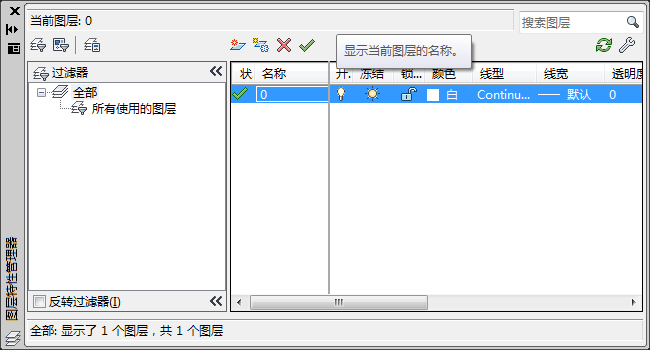
\includegraphics[scale=0.8]{Autocad_layer.png}
\caption{【图层特性管理器】对话框}\label{fig:tuchenguanliqi}
\end{figure}

单击新建图层按钮
\includegraphics[scale=0.5]{xinjiantuchen.png},新建一
\subsection{绘制图样}
\endinput
